%%%%%%%%%%%%%%%%%%%%%%%%%%%%%%%%%%%%%%%%%%%%%%%%%%%%%%%%%%%%%%%%%%%%%%%%
%                                                                      %
%     File: Thesis_Implementation.tex                                  %
%     Tex Master: Thesis.tex                                           %
%                                                                      %
%     Author: Andre C. Marta                                           %
%     Last modified :  2 Jul 2015                                      %
%                                                                      %
%%%%%%%%%%%%%%%%%%%%%%%%%%%%%%%%%%%%%%%%%%%%%%%%%%%%%%%%%%%%%%%%%%%%%%%%

\chapter{Implementation}
\label{chapter:implementation}

This section will go in depth on the implementation of the concepts presented in the chapter \ref{chapter:background}. The plane model to be controlled was firstly implemented and verified. The first goal after this first step was to design a controller that would allow the aircraft to follow a trajectory from several position waypoints through time. The influence of certain parameters and knowledge of the exact plane model will be studied and discussed in chapter \ref{chapter:results}. The final goal will be to improve the controller and its robustness by reducing tracking error through the use of an adaptive neural network.

%%%%%%%%%%%%%%%%%%%%%%%%%%%%%%%%%%%%%%%%%%%%%%%%%%%%%%%%%%%%%%%%%%%%%%%%
\section{Plane Model}
\label{section:model}

The chosen commercial aircraft that will be simulated is the Boeing 737-200, an aircraft with over 30 years of service for which information of flight parameters is readily available. The simulation was made in a cruise flight environment, at $200$ m/s velocity at $10000$ m above the ground. The chosen inertial matrix for this aircraft is given by
\begin{equation}
\begin{bmatrix}
1278369.56 & 0 & -135588.17\\
0 & 3781267.79 & 0\\
-135588.17 & 0 & 4877649.98
\end{bmatrix}
\end{equation}
The ISA atmospheric model was used to measure the air density at any given height.
\begin{table}[htbp]
  \centering
  \caption{Boeing 737-2 parameters}
    \begin{tabular}{rr}
    \toprule
    Weight $m$ & $52390$ kg \\
    Wing Span $b$ & $28.35$ m \\
    Wing Area $S$ & $102.0$ m$^{2}$ \\
    Wing mean chord $\bar{c}$ & $4.35$ m \\
    Length $l$ & $30.53$ m \\
    \bottomrule
    \end{tabular}%
  \label{tab:b737_parameters}
\end{table}%
The time constants used for the actuators was $\xi_{\delta_i}50$ms and $\xi_T=4$s for the engines.
\subsection{Plane Dynamics}
\label{section:model/plane_dynamics}

In order to simulate the aircraft's fast dynamics, its moments must firstly be computed in order to use equation \ref{eq:fast_dynamics}. The torque caused by the actuators as modelled as equation \ref{eq:cdelta}, using
\begin{gather*}
C_{L_{\delta_{ail}}}=0.02 \quad rad^{-1}\\
C_{L_{\delta_{rud}}}=0.002 \quad rad^{-1}\\
C_{M_{\delta_{ele}}}=-0.003 \quad rad^{-1}\\
C_{N_{\delta_{ail}}}= -0.002 \quad rad^{-1}\\
C_{N_{\delta_{rud}}}= -0.07 \quad rad^{-1}
\end{gather*}
The remaining aerodynamic coefficients from equation \ref{eq:cmoment} were obtained from the work of Hector Escamilla Nuñez in \cite{hector}. In this work, neural networks were used to interpolate data from the USAF Stability and Control Digital Data Compendium. A two layer feed forward network, with a hidden sigmoid activation function and a linear output activation function, was then trained using the gathered data with the Bayesian Regulation training algorithm \cite{hector}. Indeed as stated previously, neural networks can approximate any continuous function according to the Universal Approximation Theorem. This method is therefore optimal to accurately approximate the variation of these coefficients that mainly vary with the angle of attack $\alpha$ and airspeed $V_a$. The only exception to this method was the drag coefficient, given for this aircraft by
\begin{equation}
C_D=0.0176+0.0515 C_L^2
\label{eq:cd_cl}
\end{equation}

The sum of the moments can be computed and used to obtain the rotation rates $p$, $q$ and $r$. Equation \ref{eq:euler2omega} can also be used and integrated to obtain the Euler angles. These will also be necessary for frame of reference changes, namely from body to earth and vice-versa. The aerodynamic forces were computed from equation \ref{eq:forces} using the outputs of the neural networks. The body forces and acceleration relative to the earth frame were then obtain from equations \ref{eq:body_forces} and \ref{eq:boddy_acc}. 
The effects of the wind were also taken into account by adding the wind speed to the integration of the acceleration of the aircraft relative to the earth as per \ref{eq:windtriangle}. At this point the values of $\alpha$ and $\beta$ were also obtained for their respective equations \ref{eq:alpha} and \ref{eq:beta}. 

A simplified block diagram of the plane simulator is given by figure \ref{fig:plane_model}.
\begin{figure}[!htb]
  \centering
  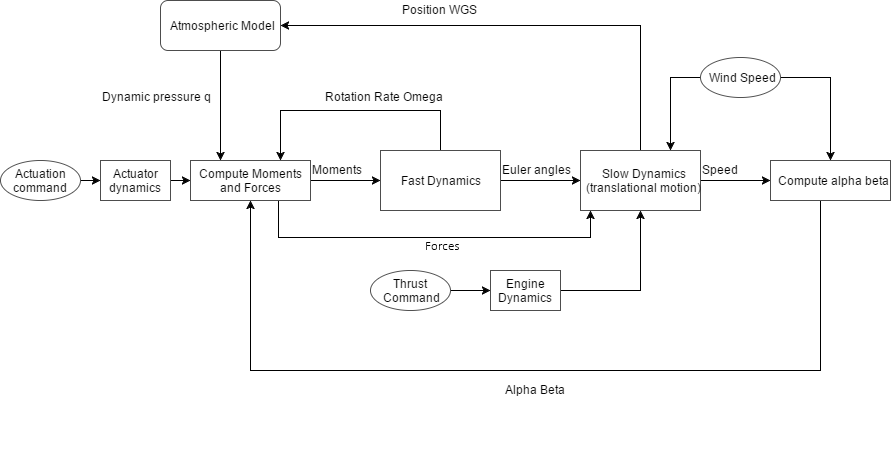
\includegraphics[width=0.75\textwidth]{Figures/PlaneModel.png}
  \caption[Plane dynamics simulator diagram]{Plane dynamics simulator diagram}
  \label{fig:plane_model}
\end{figure}
 

\section{Controller Implementation}
\label{section:control_implement}

To invert such a complex system, two layers of inversion are proposed by H. Escamilla \cite{hector}, namely for the fast and slow dynamics. Directly controlling these are three of the four actuator control inputs, the control surfaces for the aileron, elevon and rudder. These will therefore be the output of the nonlinear inversion control. To invert the fast dynamics the equation \ref{eq:fast_dynamics} must be differentiated once, to account for both the actuator dynamics \ref{eq:actuator_dynamics} and the effects of the wind. Doing so yields the jerk vector given by, as per \cite{hector}

\begin{equation}
\begin{bmatrix}
\ddot{p}\\
\ddot{q}\\
\ddot{r}
\end{bmatrix}
= \dfrac{1}{2}\rho SI^{-1} \left\lbrace V_a^2 C_\delta \xi
\begin{bmatrix}
\delta^d_{ail}-\delta_{ail}\\
\delta^d_{ele}-\delta_{ele}\\
\delta^d_{rud}-\delta_{rud}
\end{bmatrix}
+V_a^2C_c\dot{R_a}+2V_a\dot{V_a}\left(
\begin{bmatrix}
bC_l\\
\bar{c}C_m\\
bC_n
\end{bmatrix}
+ C_\delta 
\begin{bmatrix}
\delta_{ail}\\
\delta_{ele}\\
\delta_{rud}
\end{bmatrix}
\right) \right \rbrace + I^{-1}\left(\dfrac{1}{4}\rho SV_aC_k-In\right)\dot{\Omega}
\label{eq:jerk}
\end{equation}

Where

\begin{gather*}
I=
\begin{bmatrix}
A & 0 & -E\\
0 & B & 0\\
-E & 0 & C
\end{bmatrix}\\
I_n=
\begin{bmatrix}
-Eq & (C-B)r-Ep & (C-B)q\\
(A-C)r+2Ep & 0 & (A-C)p-2Er\\
(B-A)q & (B-A)p+Er & Eq
\end{bmatrix}\\
\xi=
\begin{bmatrix}
\dfrac{1}{\xi_{ail}} & 0 & 0\\
0 & \dfrac{1}{\xi_{ele}} & 0\\
0 & 0 & \dfrac{1}{\xi_{rud}}
\end{bmatrix}\\
C_c=
\begin{bmatrix}
0 & bC_{l_\beta} & -\dfrac{b^2}{2V_a^2}(C_{l_p}p+C_{l_r}r)\\
\bar{c}C_{m_\alpha} & 0 & -\dfrac{\bar{c}^2}{2V_a^2}C_{m_q}q\\
0 & bC_{n_\beta} & -\dfrac{b^2}{2V_a^2}(C_{n_p}p+C_{n_r}r)
\end{bmatrix}\\
C_k=
\begin{bmatrix}
b^2C_{l_p} & 0 & b^2C_{l_r}\\
0 & \bar{c}^2C_{m_q} & 0\\
b^2C_{n_p} & 0 & b^2C_{n_r}
\end{bmatrix}\\
\dot{Ra} =  [\dot{\alpha} \quad \dot{\beta} \quad \dot{V_a}]^T
\end{gather*}

To do a feedback linearisation, a pseudo input must be chosen, in this case $\tau = \ddot{\Omega}$. The feedback control law will therefore be, solving equation \ref{eq:jerk} to $\delta^d$,

\begin{equation}
\begin{bmatrix}
\delta^d_{ail}\\
\delta^d_{ele}\\
\delta^d_{rud}
\end{bmatrix}
=\dfrac{1}{V_a^2}\xi^-1C_\delta\left\lbrace\dfrac{2I}{\rho S}\tau - \dfrac{2}{\rho S}(\dfrac{1}{4}\rho S V_aC_k - I_n)\dot{\Omega} -2V_a\dot{V_a} \left(
\begin{bmatrix}
bC_l\\
\bar{c}C_m\\
bC_n
\end{bmatrix}
+ C_\delta \delta\right)-V_a^2C_c\dot{R_a} \right\rbrace+ \delta
\end{equation}

(Check if conditions from MIMO NLI are respected)

The wind effects will appear in the terms including $\dot{Ra} =  [\dot{\alpha} \quad \dot{\beta} \quad \dot{V_a}]^T$, as the equation defining $\dot{V_a}$ can be obtained differentiating the norm of the speed relative to the ground. SEE ANNEX HERE 

Should all of the parameters mentioned in the equations above be known and no inversion error be made, the resulting system $\Omega=\tau$ will be both linear and decoupled, having three pseudo inputs $\tau = [\tau_p \quad \tau_q \quad \tau_r]_T$. As mentioned in section \ref{section:background/NLI}, the next step of the nonlinear inversion shall be to propose a linear controller for this resulting system. Taking the desired rotation rates $\Omega^d$ as inputs comes a control law for $\tau$, firstly considering without neural network adaptation
\begin{equation}
\tau = -K_P (\Omega-\Omega^d)-K_D (\dot{\Omega}-\dot{\Omega}^d)+\ddot{\Omega}
\label{eq:linear_controller}
\end{equation}
Where the $K_P$ and $K_D$ coefficients are chosen to assure stability of KD NOT EMPIRICALLY?

From this point the next step shall be to obtain the desired values of $\Omega$. These were obtained using another PD controller, using Euler angle reference values to control rotation rates. Among these reference values to be followed, $\tau_r$ was set to zero. This was made to make use of the decoupling through feedback linearisation of the plane's movement, using a roll and pitch motion to turn the aircraft. This results in the following control of rotation rate
\begin{subequations}
\begin{equation}
p= k_P (\phi^d-\phi) + k_d (\dot{\phi^d-\dot{\phi}})
\end{equation}
\begin{equation}
q= k_P (\theta^d-\theta) + k_d (\dot{\theta^d-\dot{\theta}})
\end{equation}
\begin{equation}
r=0
\end{equation}
\end{subequations}
\section{Neural Network}
\label{section:NN}

\section{Verification and Validation}
\label{section:model/verification}

The goal in this section will be to validate the behaviour of the model in cruise conditions. Assuming cruise conditions comes that

\begin{gather}
	T=D\\
	W=L\\
	L'=M=N=0
\label{eq:cruise_cond}
\end{gather}
In order to verify the model described so far, the required thrust to have cruise conditions will be computed for a given plausible value of $\alpha$. From this point the airspeed of the aircraft can also be computed. The graph of $C_L$ versus alpha was also obtained from its respective neural network, given by \ref{fig:cl_alpha}
\begin{figure}[!htb]
  \centering
  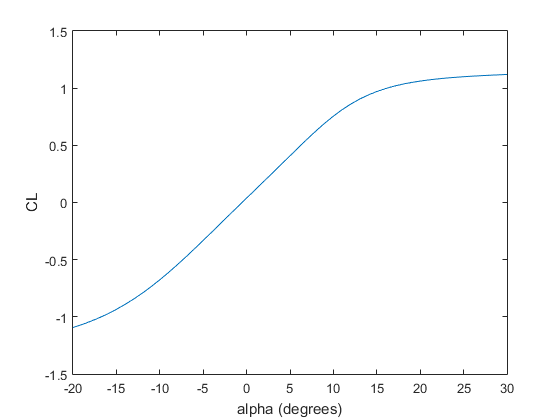
\includegraphics[width=1\textwidth]{Figures/CL_alpha.png}
  \caption[$C_L$ versus $\alpha$ graph]{$C_L$ versus $\alpha$ graph from Neural Network}
  \label{fig:cl_alpha}
\end{figure}
From the cruise conditions \ref{eq:cruise_cond}, knowing that $L=\dfrac{1}{2}\rho S V^2 C_L$, solving for the airspeed V comes that

\begin{equation}
V=\sqrt{\dfrac{2mg}{\rho S C_L}}
\label{eq:cruise_speed}
\end{equation}
The required thrust can also be computed from both \ref{eq:cruise_cond}, \ref{eq:cruise_speed} and \ref{eq:cd_cl}, knowing the $C_L$ for a given angle of attack. Proposing some values of $\alpha$, the following results are obtained

\begin{table}[htbp]
  \centering
  \caption{Required cruise conditions for different values of $\alpha$}
    \begin{tabular}{ccccc}
    \toprule
    $\alpha (^o)$ & $C_D$ & $C_L$ & $V (ms^{-1})$ & $T (N)$ \\
    \midrule
    0     & 0.017677131 & 0.0387 & 707.4010791 & 224047.3585 \\
    2     & 0.019379779 & 0.1859 & 322.7613368 & 51133.84325 \\
    4     & 0.023345134 & 0.334 & 240.7952785 & 34283.79709 \\
    6     & 0.029604436 & 0.4828 & 200.279994 & 30076.58604 \\
    \bottomrule

    \end{tabular}%
  \label{tab:cruise_cond}%
\end{table}%
